\section{LLM Economist}
\label{sec:llm_economist}

The \textit{LLM Economist} realizes the Stackelberg game of Section~\ref{sec:preliminaries} with language-based agents that act purely \emph{in-context}.  Simulator state, history, and objectives are rendered as text; actions are JSON snippets parsed by the environment.  This design unifies in-context reinforcement learning, census-grounded population modeling, and dynamic tax-mechanism optimization within a single framework.

\paragraph{In-Context Reinforcement Learning.}
At each daily step \(t\) the environment serializes the joint state \(o_t\) into a prompt \(\pi_t\).  Worker \(\mathcal{W}_i\) returns \verb|{"LABOR": X}|, while at the start of tax year \(k\) the planner \(\mathcal{P}\) emits \ldots\verb|{"DELTA":[· · ·]}| specifying bracket shifts $\Delta\tau_k\in[-20,20]^B$, where each element is clipped to $\pm20$ percent to avoid unrealistically large moves and high variance. 
Prompts follow a two-phase pattern—\emph{exploration} then \emph{exploitation}—that encourages broad search before convergence.  A replay buffer keeps the best running average \(h\) state–action–welfare triples and splices them into future prompts, supplying token-level credit assignment across long horizons.

\begin{figure*}[t]
  \centering
  % \includegraphics[width=0.5\linewidth]{fig/fig1_econ.png} 
  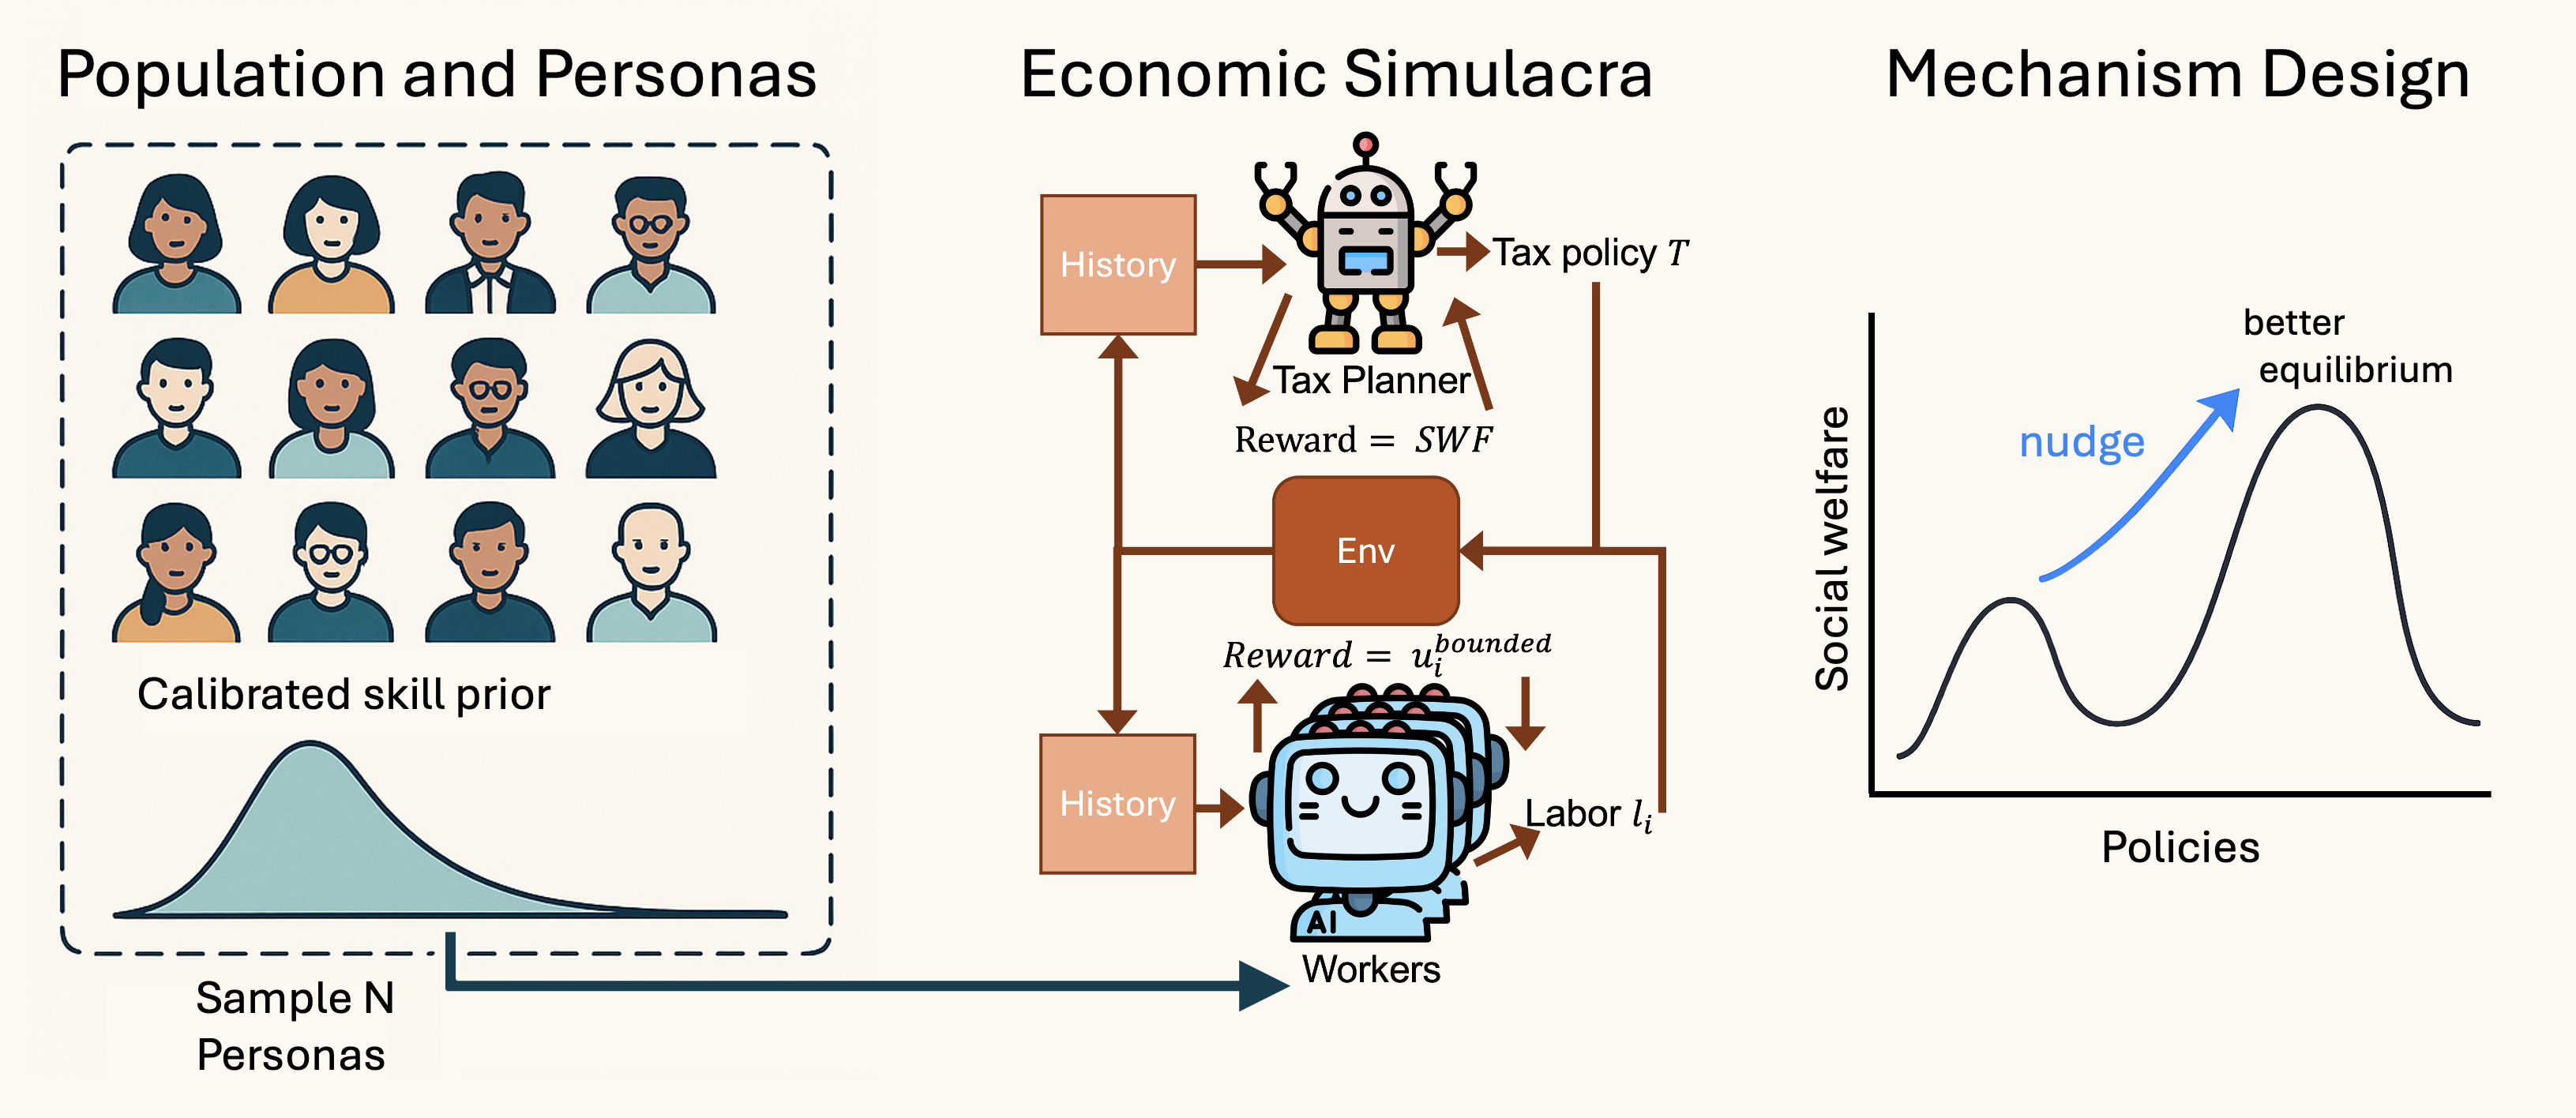
\includegraphics[width=0.9\linewidth]{fig/llm_econ_fig1.png}
  \caption{\textbf{Overview of the \emph{LLM Economist}.}
  % \emph{Left:} a population of persona-conditioned language agents instantiated from an ACS-calibrated skill prior.  \emph{Right:} the two-level in-context reinforcement-learning architecture.  At the lower tier each worker LLM receives a text history, selects labor $\ell_i$, and receives a bounded utility reward $u_i^{\text{bounded}}$. At the upper tier the planner LLM observes an aggregated history, proposes a marginal tax schedule $T$, and receives social-welfare feedback $\mathrm{swf}$.  The shared environment mediates tax payments, rebates, and state transitions, while the token-level reward stream closes the learning loop for both tiers. Iterating over text observation $\rightarrow$ LLM $\rightarrow$ JSON action $\rightarrow$ environment drives the system toward the Stackelberg equilibrium studied throughout the paper.}
  \emph{Left:} We draw a population of $N$ language‑based worker agents from an ACS–calibrated skill prior, instantiating each with a distinct persona.
  \emph{Center:} Inside the economic simulacrum, workers observe text histories, choose labor $l_i$, and receive utility $u_i$, while a planner agent proposes a marginal tax schedule $\tau$ to maximize social welfare $\texttt{SWF}=\sum_i u_i/z_i$. The shared environment mediates tax collection, lump‑sum rebates, and state transitions, allowing both tiers to adapt in‑context from their respective histories. 
  \emph{Right:} Mechanism design is visualized as climbing a rugged social‑welfare landscape; successive planner “nudges’’ steer the economy toward higher‑payoff Stackelberg equilibria.}
  \label{fig:system_overview}
\end{figure*}



% \wenzhe{A bit unstructured IMO. I would suggest structure as follows: (1) design of observation space (memory module) (2) design of planner (exploration/exploitation prompt) (3) design of worker (exploration/exploitation prompt, skill population, bounded utility) (4) extended features (democratic)}

\smallskip\noindent
\textbf{Example planner exploration prompt:}\\[-0.6em]
\begin{tcolorbox}[colback=gray!10,colframe=black,sharp corners,boxrule=1pt,width=\columnwidth,left=0pt,right=0pt]
\small
Use the historical data to influence your answer in order to maximize SWF, while balancing exploration and exploitation by choosing varying rates of TAX. The best marginal tax rate historically was \texttt{TAX=[60\% 60\%]} corresponding to \texttt{SWF=1.0}. Try different rates of \texttt{TAX} before picking the one that corresponds to the highest \texttt{SWF}.
\end{tcolorbox}

\noindent
\textbf{Example worker exploitation prompt:}\\[-0.6em]
\begin{tcolorbox}[colback=gray!10,colframe=black,sharp corners,boxrule=1pt,width=\columnwidth,left=0pt,right=0pt]
\small
Decreasing labor decreased utility. This implies labor \(\ell\) is too low and needs to be increased above labor \(\ell = 10.0\).
\end{tcolorbox}

\paragraph{Observation spaces.}
Workers observe
\[
o_t^i=\bigl(z_t^i,\hat z_t^i,\tau_{\lfloor t/K\rfloor}(z_t^i),R_t,
           \text{history window}\bigr),
\]
where \(z_t^i=s^i l_t^i\) and \(\hat z_t^i\) is post-tax income.  
The planner receives histograms of \(z\) and worker utilities, a moving average of social welfare, and the best \(h\) trajectories to date.

\paragraph{Workers: Large Population Models.}
Skills \(s^{i}\) are drawn from a generalized-Beta fit to the 2023 American Community Survey (ACS) Public-Use Microdata Sample \citep{acs2023pums}.
Demographic fields (age, occupation, gender) and a \emph{persona} string are woven into each system prompt.  An example persona is shown below.

\begin{tcolorbox}[colback=gray!10,colframe=black,sharp corners,boxrule=1pt,width=\columnwidth,left=0pt,right=0pt]
\small
You're a 32-year-old entrepreneur running a small tech startup. You work 60+ hours a week, pouring your energy into building your business. You believe that lower taxes let you reinvest in your company, hire more employees, and secure your financial future. For you, higher taxes feel like a punishment for success. While you appreciate government services, you feel efficiency and accountability are lacking in how tax dollars are spent.
\end{tcolorbox}

The \textsc{isoelastic} scenario uses a rational (isoelastic) utility function,
\begin{equation}\label{eq:isoelastic}
u(\hat z,l)=\frac{\hat z^{1-\eta}-1}{1-\eta}-\psi\,l^{\delta},
\end{equation}
with risk-aversion $\eta$ and labor-disutility parameters $\psi,\delta$. 

In the \textsc{bounded} scenario, worker \(i\) computes a satisfaction flag \(s_t^i\in\{0,1\}\) from \(o_t^i\).  Utility becomes
\begin{equation}\label{eq:bounded}
    u_i^{\text{bounded}}(\hat z,l)=
\frac{\hat z^{1-\eta}-1}{1-\eta}-\psi\,l^{\delta}
-\bigl(1-s_t^i\bigr)\phi,
\end{equation}
where \(\phi\) is a fixed dissatisfaction penalty calibrated so that a one-bracket misalignment reduces utility by half.

\paragraph{Planner: Designing a Tax Mechanism.}
The planner starts from a flat schedule or the US schedule and searches over \(\Delta\tau_k\).  Its prompt stores \textit{(i)} income and utility histograms, \textit{(ii)} the last \(h\) social-welfare values, and \textit{(iii)} the best tax vector observed so far.   After applying \(\Delta\tau_k\) the environment computes a rebate \(R_t\) that redistributes to the population.

\paragraph{Additional action: Democratic voting.} 
In the \textsc{democratic} setting, workers vote at year-end to keep the incumbent planner or replace it with a challenger sampled from a language-model prior; the candidates create text platforms to convince workers. The winner’s prompt history carries forward.

% \begin{figure}[t]
%   \centering
%   \includegraphics[width=\linewidth]{fig/llm_economist_arch}
%   \caption{\textbf{Architecture of the LLM Economist.}  The planner (top) updates the marginal tax schedule once per tax year, conditioning on aggregated statistics from the worker layer (bottom).  Workers receive persona-specific prompts, choose labor, and receive rebates.  Dashed arrows show information flow; solid arrows denote actions.}
%   \label{fig:llm_economist_arch}
% \end{figure}

% The next section details training protocols and baselines; empirical results appear in Section~\ref{sec:experiments}.
As we shall see later in the next section, our design of the LLM Economist enables effective in-context RL for both planner and workers, empowering LLMs to make informative and beneficial tax decisions, and extending the application of LLM-based simulacra to studying emergent behaviors of agents.
